\documentclass[rgb]{beamer}

\usepackage[english]{babel}
\usepackage[utf8]{inputenc}
\usepackage{xcolor}
\usepackage{listings}
\usepackage{adjustbox}
\usepackage{amsmath}
\usepackage{multirow}
\usepackage[linewidth=1pt]{mdframed}

% Graphics
\usepackage{graphicx}

\usepackage{tikz}
\usetikzlibrary{calc,shapes.multipart,chains,arrows}

% Font
\usepackage{paratype}
\setbeamerfont{frametitle}{family=\bf}

% Beamer theme settings
\usecolortheme{seagull}
\setbeamertemplate{itemize item}{\raisebox{0.8mm}{\rule{1.8mm}{1.2mm}}}
\usenavigationsymbolstemplate{} % no navigation buttons

\usepackage{listings}

% Define Language
\lstdefinelanguage{fsharp}
{
  % list of keywords
  morekeywords={
    and,
    do,
    else,
    exception,
    for,
    fun,
    function,
    if,
    in,
    let,
    match,
    module,
    mutable,
    open,
    of,
    rec,
    then,
    try,
    type,
    unsafe,
    use,
    val,
    when,
    while,
    with,
  },
  sensitive=true, % keywords are not case-sensitive
  morecomment=[l]{//}, % l is for line comment
%  otherkeywords={>,<,=,<=,>=,!,*,/,-,+,|,&,||,&&,==,=>},
  morestring=[b]" % defines that strings are enclosed in double quotes
}

% Define Colors
\usepackage{color}
\definecolor{eclipseBlue}{RGB}{42,0.0,255}
\definecolor{eclipseGreen}{RGB}{63,127,95}
\definecolor{eclipsePurple}{RGB}{127,0,85}

\newcommand{\fop}[1]{\mbox{\ttfamily\color{eclipseBlue}#1}}
\newcommand{\fw}[1]{\mbox{\ttfamily\bfseries\color{eclipsePurple}#1}}

% Set Language
\lstset{
  language={fsharp},
  basicstyle=\ttfamily, % Global Code Style
  captionpos=b, % Position of the Caption (t for top, b for bottom)
  extendedchars=true, % Allows 256 instead of 128 ASCII characters
  tabsize=2, % number of spaces indented when discovering a tab
  columns=fixed, % make all characters equal width
  keepspaces=true, % does not ignore spaces to fit width, convert tabs to spaces
  showstringspaces=false, % lets spaces in strings appear as real spaces
  breaklines=true, % wrap lines if they don't fit
  frame=trbl, % draw a frame at the top, right, left and bottom of the listing
  frameround=tttt, % make the frame round at all four corners
  framesep=4pt, % quarter circle size of the round corners
  numbers=left, % show line numbers at the left
  numberstyle=\small\ttfamily, % style of the line numbers
  commentstyle=\slshape\bfseries\color{eclipseGreen}, % style of comments
  keywordstyle=\bfseries\color{eclipsePurple}, % style of keywords
  stringstyle=\color{eclipseBlue}, % style of strings
  emph=[1] {
    false,
    true,
    Set,
    Map,
    List,
    ImgUtil,
    Pegs,
    String,
    Array,
    Array2D
  },
  emphstyle=[1]{\color{eclipseBlue}},
  moredelim=**[is][\color{red}]{@@}{@@}
}

\newcommand{\theyear}{2020}
\newcommand{\sem}[1]{[\![#1]\!]}
\newcommand{\seme}[1]{\sem{#1}\varepsilon}
\newcommand{\semzero}[1]{\sem{#1}_0}

\newcommand{\emptymap}{\{\}}
\newcommand{\fracc}[2]{\begin{eqnarray} \frac{\begin{array}{c} #1
    \end{array}}{\begin{array}{c} #2 \end{array}} \end{eqnarray}}
\newcommand{\sembox}[1]{\hfill \normalfont \mbox{\fbox{\(#1\)}}}
\newcommand{\sempart}[2]{\subsubsection*{\rm\em #1 \sembox{#2}}}
\newcommand{\axiom}[1]{\begin{eqnarray} \begin{array}{c} #1 \end{array} \end{eqnarray}}
\newcommand{\fraccn}[2]{\refstepcounter{equation}\mbox{$\frac{\begin{array}{c} #1 \end{array}}{\begin{array}{c} #2 \end{array}}$}~(\arabic{equation})}
\newcommand{\fraccc}[2]{\mbox{$\frac{\begin{array}{c} #1 \end{array}}{\begin{array}{c} #2 \end{array}}$}}
\newcommand{\onepart}[1]{\noindent\hfill#1\hfill~\vspace{2mm}}
\newcommand{\twopart}[2]{\noindent\hfill#1\hfill#2\hfill~\vspace{2mm}}
\newcommand{\threepart}[3]{\noindent\hfill#1\hfill#2\hfill#3\hfill~\vspace{2mm}}
%\newcommand{\axiomm}[1]{\refstepcounter{equation}\mbox{$\begin{array}{c} #1 \end{array}$}~(\arabic{equation})}
\newcommand{\axiomm}[1]{$\begin{array}{c} #1 \end{array}$}
%\newcommand{\ar}[1]{\stackrel{#1}{\longrightarrow}}
\newcommand{\vd}{\vdash}
\newcommand{\Ran}{{\rm Ran}}
\newcommand{\Dom}{{\rm Dom}}
\newcommand{\kw}[1]{\texttt{#1}}
\newcommand{\id}[1]{\mbox{\it{#1}}}
\newcommand{\rarr}{\rightarrow}
\newcommand{\eval}{\rarr}
\newcommand{\evals}{\leadsto}
\newcommand{\larr}{\leftarrow}

\newcommand{\head}[1]{\vspace{3mm} \textbf{\normalsize #1}}
\newcommand{\headsp}[1]{\head{#1}\vspace{1ex}}
\newcommand{\size}{\ensuremath{\mathrm{size}}}
\renewcommand{\log}{\ensuremath{\mathrm{log}}}

\newcommand{\setallthemecolors}[1]{%
\setbeamercolor*{palette primary}{use=structure,fg=white,bg=#1}%
\setbeamercolor*{palette secondary}{use=structure,fg=white,bg=#1}%
\setbeamercolor*{palette tertiary}{use=structure,fg=white,bg=#1}}

\definecolor{black}{RGB}{0,0,0}
\definecolor{maroon}{RGB}{128,0,0}
\definecolor{olive}{RGB}{128,128,0}
\definecolor{green}{RGB}{0,128,0}
\definecolor{purple}{RGB}{128,0,128}
\definecolor{teal}{RGB}{0,128,128}
\definecolor{darkteal}{RGB}{0,92,92}
\definecolor{navy}{RGB}{0,0,128}
\definecolor{gray}{RGB}{128,128,128}
\definecolor{darkgray}{RGB}{60,60,60}
\definecolor{darkred}{RGB}{139,0,0}

%palette

% #173F5F (dark blue)
\definecolor{darkblue}{RGB}{23,63,95}
% #20639B (blue)
\definecolor{blue}{RGB}{32,99,155}
% #3CAEA3 (green)
\definecolor{magenta}{RGB}{60,174,163}
% #F6D55C (yellow)
\definecolor{yellow}{RGB}{246,213,92}
% #ED553B (red)
\definecolor{red}{RGB}{237,85,59}


\usecolortheme{whale}
\useoutertheme{infolines}
\useinnertheme{rectangles}

\newcommand{\popsettitle}[2]{%
\setallthemecolors{#1}%
\newcommand{\popemne}{#2}%
\title{Programmering og Problemløsning}%
\subtitle{#2}%
\author{Martin Elsman}%
\date{}%
\institute[DIKU]{Datalogisk Institut, Københavns Universitet (DIKU)}}

\newcommand{\popmaketitleframe}{%
  \frame{\titlepage%
   \vspace{-15mm}%
   \par\noindent\rule{\textwidth}{0.4pt}%

   \vspace{4mm}%
   \tableofcontents%
   \vspace{-4mm}%
   \par\noindent\rule{\textwidth}{0.4pt}%
  }%
  \section*{\popemne}%
}


\popsettitle{darkblue}{Programmering med Arrays}

\begin{document}

\popmaketitleframe

%%%%%%%%%%%%%%%%%%%%%%%%%%%%%%%%%%%%%%%%%%%%%%%%
\subsection{1D Arrays}
%%%%%%%%%%%%%%%%%%%%%%%%%%%%%%%%%%%%%%%%%%%%%%%%

\begin{frame}[fragile]

\headsp{Introduktion til 1D arrays}

\textbf{Syntax}

\begin{lstlisting}[numbers=none,frame=none]
  let arr : int [] = [|1;2;3;4|]
\end{lstlisting}

\textbf{Lagerrepræsentation}

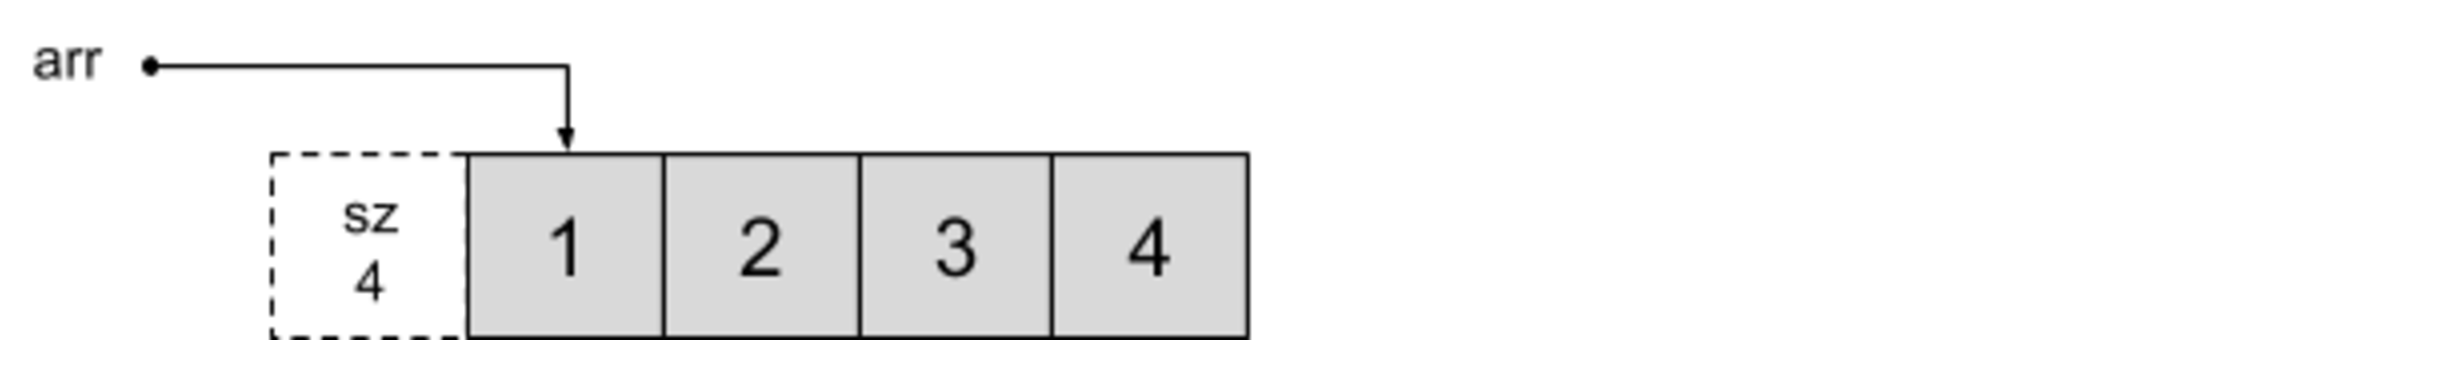
\includegraphics[width=0.9\textwidth]{array1234.png}

\textbf{Bemærk}

\begin{itemize}
  \item Det er \textbf{IKKE} nemt at tilføje ekstra elementer.
  \item Det er nemt (hurtigt) at læse ethvert element i et array.

  \item Arrays er \emph{mutable}, dvs det er muligt (hurtigt) at
    opdatere ethvert element.
  \end{itemize}
\end{frame}

%%%%%%%%%%%%%%%%%%%%%%%%%%%%%%%%%%%%%%%%%%%%%%%%
\subsection{Gennemløb af 1D arrays}
%%%%%%%%%%%%%%%%%%%%%%%%%%%%%%%%%%%%%%%%%%%%%%%%

\begin{frame}[fragile]
\begin{footnotesize}
\headsp{Gennemløb af 1D arrays}

Arrays kan gennemløbes tilsvarende som lister:

\vspace{1ex}

\begin{lstlisting}[numbers=none,frame=none,mathescape]
let arr = Array.init 50000 (fun x -> x)
let mutable sum = 0
for x in arr do sum <- sum + x
do printf "%d\n" sum
\end{lstlisting}

\vspace{1ex}
\headsp{Arrays kan muteres}

\begin{lstlisting}[numbers=none,frame=none,mathescape]
let arr = [|1;2;3;4|]
for i in [0..arr.Length-1] do arr.[i] <- arr.[i]*arr.[i]
do printf "%A\n" arr
\end{lstlisting}

\vspace{1ex}
\head{Kørsel:}

\begin{verbatim}
bash-3.2$ fsharpc --nologo arr_square.fs && mono arr_square.exe
[|1; 4; 9; 16|]
\end{verbatim}
\end{footnotesize}
\end{frame}

%%%%%%%%%%%%%%%%%%%%%%%%%%%%%%%%%%%%%%%%%%%%%%%%
\subsection{Array aliasing}
%%%%%%%%%%%%%%%%%%%%%%%%%%%%%%%%%%%%%%%%%%%%%%%%

\begin{frame}[fragile]
\begin{footnotesize}
\head{Array aliasing}

\vspace{1ex}

To forskellige variabler kan referere til det samme array:
\begin{lstlisting}[numbers=none,frame=none,mathescape]
let arr = [|1;2;3;4|]
let b = arr
do b[1] <- 100
do printf "%A\n" arr
\end{lstlisting}

\vspace{1ex}
\head{Lagerrepræsentation:}
\vspace{1ex}

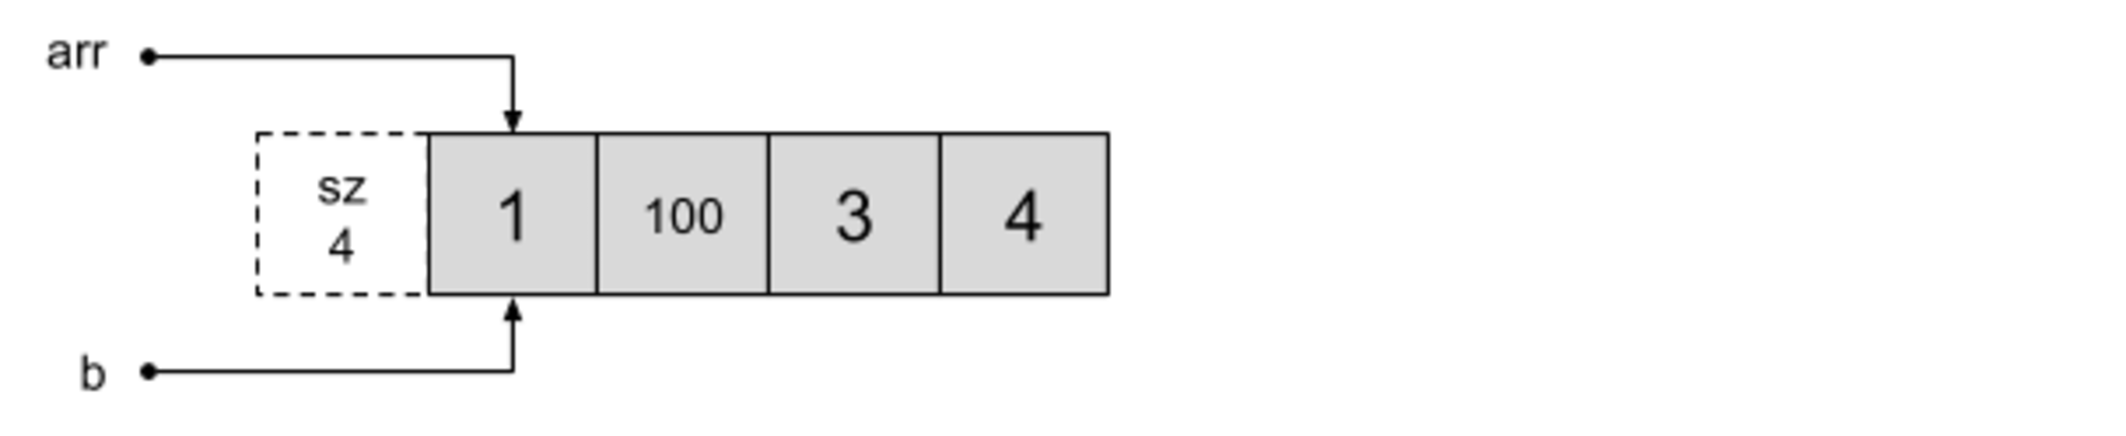
\includegraphics[width=0.9\textwidth]{arr_b_1234.png}

\vspace{1ex}
\head{Bemærk:}
\begin{enumerate}
\item Aliasing kan observeres fordi arrays er mutable!
\item Aliasing (og deling) kan ikke observeres (på samme måde) med lister, da disse er immutable.
\end{enumerate}

\end{footnotesize}
\end{frame}

%%%%%%%%%%%%%%%%%%%%%%%%%%%%%%%%%%%%%%%%%%%%%%%%
\subsection{Modulet \lstinline{Array}}
%%%%%%%%%%%%%%%%%%%%%%%%%%%%%%%%%%%%%%%%%%%%%%%%

\begin{frame}[fragile]
\begin{footnotesize}
\head{Modulet \lstinline{Array}}
\vspace{1ex}
\begin{lstlisting}[numbers=none,frame=none]
// array creation
val init     : int -> (int -> 'a) -> 'a []
val length   : 'a [] -> int   // length a = a.Length
val toList   : 'a [] -> 'a list
val ofList   : 'a list -> 'a []

// array transformers
val map      : ('a -> 'b) -> 'a [] -> 'b []
val map2     : ('a->'b->'c) -> 'a [] -> 'b [] -> 'c []
val filter   : ('a -> bool) -> 'a [] -> 'a []

// array traversing
val fold     : ('a -> 'b -> 'a) -> 'a -> 'b [] -> 'a
val foldBack : ('b -> 'a -> 'a) -> 'b [] -> 'a -> 'a
val find     : ('a -> bool) -> 'a [] -> 'a
...
\end{lstlisting}

\end{footnotesize}
\end{frame}

\begin{frame}[fragile]
\begin{footnotesize}
\head{Array reverse}
\vspace{1ex}

Her følger et første forsøg på at vende et array om (ved brug af
mutation):

\begin{lstlisting}[numbers=none,frame=none]
let badrev (arr: int[]) : unit =
  for i in [0..arr.Length-1] do
    arr.[i] <- arr.[arr.Length-i-1]

let arr = [|1;2;3;4|]
do badrev arr
do printf "%A\n" arr
\end{lstlisting}

\head{Spørgsmål?}
\begin{itemize}
\item Hvad er der galt med \kw{badrev}?
\item Hvad er indholdet af \kw{arr} efter kaldet til \kw{badrev}?
\end{itemize}

\end{footnotesize}
\end{frame}

\begin{frame}[fragile]
\begin{footnotesize}
\head{Array reverse (fortsat)}
\vspace{1ex}

Here er et bedre forsøg:

\begin{lstlisting}[numbers=none,frame=none]
let rev (arr: int[]) : unit =
  for i in [0..arr.Length/2-1] do
    let tmp = arr.[i]
    do arr.[i] <- arr.[arr.Length-i-1]
    do arr.[arr.Length-i-1] <- tmp;;

let arr = [|1;2;3;4|]
do rev arr
do printf "%A\n" arr

let arr = [|1;2;8;3;4|]
do rev arr
do printf "%A\n" arr
\end{lstlisting}

\head{Bemærk:}
\begin{itemize}
\item Vi benytter os af en temporær variabel til at holde indholdet af
  et array element før det overskrives.
\item Funktionen gør brug af en swap-strategi.
\end{itemize}

\end{footnotesize}
\end{frame}

%%%%%%%%%%%%%%%%%%%%%%%%%%%%%%%%%%%%%%%%%%%%%%%%
\subsection{2D Arrays}
%%%%%%%%%%%%%%%%%%%%%%%%%%%%%%%%%%%%%%%%%%%%%%%%

\begin{frame}[fragile]
\begin{footnotesize}
\head{To-dimensionelle arrays}
\vspace{1ex}

To-dimensionelle \emph{regulære arrays} (dvs. 2d-arrays hvor alle
rækker indeholder \hspace{2cm} det samme antal elementer) kan håndteres ved brug af
modulet \lstinline{Array2D}.

\vspace{1ex}

Modulet \lstinline{Array2D} kan benyttes til f.eks. at konstruere
en multiplikationstabel:

\vspace{1ex}

\begin{lstlisting}[numbers=none,frame=none]
let a = Array2D.init 5 5 (fun r c -> (r+1) * (c+1))
let prA (a : int[,]) =
  for r in [0..Array2D.length1 a - 1] do    // 1  2  3  4  5
    for c in [0..Array2D.length2 a - 1] do  // 2  4  6  8 10
      printf "%2d " (a.[r,c])               // 3  6  9 12 15
    printf "\n"                             // 4  8 12 16 20
do prA a                                    // 5 10 15 20 25
\end{lstlisting}

\head{Bemærk:}
\vspace{1ex}

\begin{enumerate}
\item Typen på et to-dimensionelt int-array skrives: \lstinline{int[,]}.
\item Vidden på de udskrevne heltal kontrolleres med format-specifieren \lstinline{"%2d "}.
\end{enumerate}
\end{footnotesize}
\end{frame}

\subsection*{Konklusion}
\begin{frame}[fragile]
  \headsp{Konklusion}

  \vspace{3mm}
  \tableofcontents
\end{frame}

\end{document}
